AutoFOCUS3 (AF3) is an open source model based development tool for distributed, reactive and embedded software systems. It uses models to develop systems. From the requirements to the hardware architecture, passing by the design of the logical architecture, the deployment and the scheduling. It provides advanced features to support the user ensuring the quality of their system: formal analyses, synthesis methods, space exploration visualization, etc.

Co-simulation feature supports for now only Functional Mockup Unit (FMU) export satisfying the following constraints:
\begin{itemize}
  \item FMI 2.0
  \item 32/64bit
  \item GCC compilation
  \item Input and output values cannot carry NoVal but instead contain default values (0 for integers and reals, false for booleans, first item for enumerations) Note: This behavior is different from AF3 simulation
\end{itemize}

FMI export is done at the level of component with logical architecture (in the future, we might implement this feature for deployments as well). To export your component with logical architecture to the  FMU, right-click on it in the model navigator and select "Export to FMU2.0" as shown in \autoref{figure:autoFOCUSFMUExport}.

\begin{figure}[ht]
	\centerline{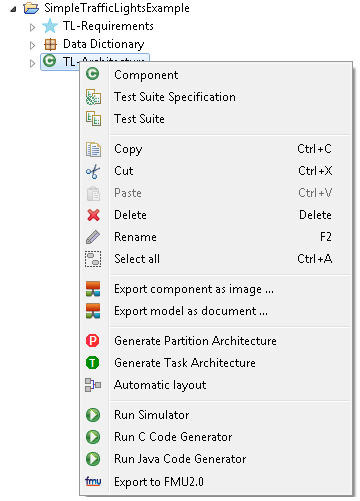
\includegraphics[width=0.6\textwidth]{figures/autoFOCUSFMUExport.png}}
	\caption{Exporting component architecture to FMU.}
	\label{figure:autoFOCUSFMUExport}
\end{figure}

AF3 works with logical time, however co-simulation is generally achieved with tools modeling reality and therefore working with real time. Therefore, the FMI standard requires that AF3 notion of time is translated to real time. Consequently, you will have to define the sampling time (in seconds) for the component as a function with name "samplingTime()" in the data dictionary as shown in \autoref{figure:autoFOCUSSamplingTime}. Otherwise, you will be asked to provide the frequency of the component in Hertz as shown in  \autoref{figure:autoFOCUSFrequency}.

\begin{figure}[ht]
	\centerline{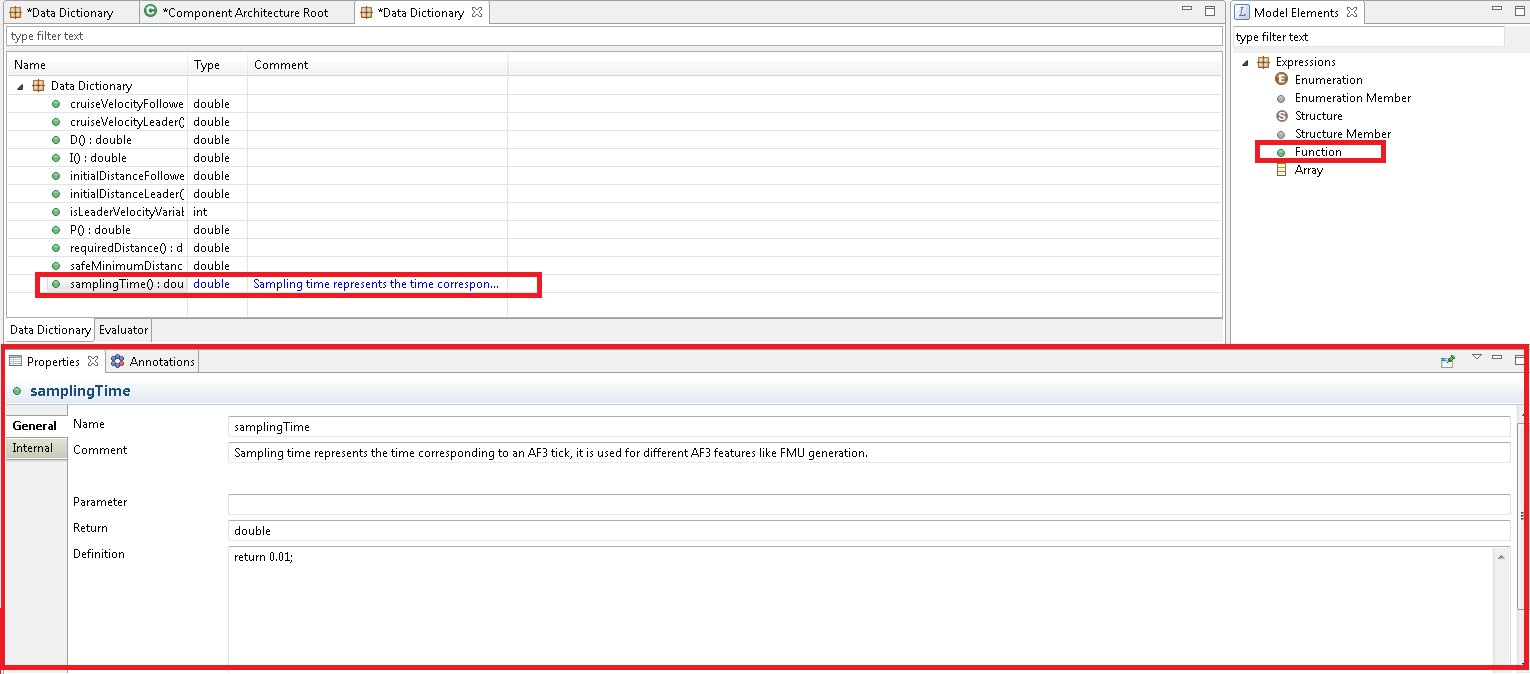
\includegraphics[width=1\textwidth]{figures/autoFOCUSSamplingTime.png}}
	\caption{Defining the sampling time function in data dictionary.}
	\label{figure:autoFOCUSSamplingTime}
\end{figure}

\begin{figure}[ht]
	\centerline{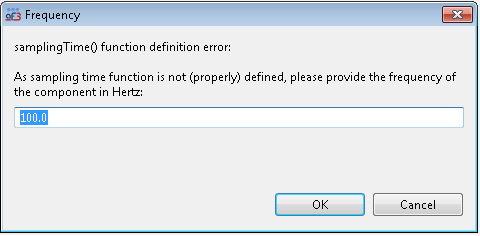
\includegraphics[width=0.6\textwidth]{figures/autoFOCUSFrequency.png}}
	\caption{Providing the component frequency in case of samplingtime() function not defined.}
	\label{figure:autoFOCUSFrequency}
\end{figure}


